\documentclass[10pt]{article}
\usepackage[polish]{babel}
\usepackage[utf8]{inputenc}
\usepackage[T1]{fontenc}
\usepackage{amsmath}
\usepackage{amsfonts}
\usepackage{amssymb}
\usepackage[version=4]{mhchem}
\usepackage{stmaryrd}
\usepackage{graphicx}
\usepackage[export]{adjustbox}
\graphicspath{ {./images/} }

\title{LIGA MATEMATYCZNA \\
 im. Zdzisława Matuskiego GRUDZIEŃ 2021 SZKOŁA PODSTAWOWA \\
 klasy IV - VI }

\author{}
\date{}


\begin{document}
\maketitle
\section*{ZADANIE 1.}
Numer mieszkania Mikołaja jest liczbą dwucyfrową podzielną przez 13, a po dodaniu do numeru mieszkania liczby 1 dostajemy wielokrotność liczby 11. Wyznacz sumę cyfr numeru mieszkania Mikołaja.

\section*{ZADANIE 2.}
Obwód pięciokąta wypukłego \(A B C D E\) jest równy 82 . Obwód czworokąta \(A B C D\) wynosi 64 , a obwód czworokąta \(A C D E\) równa się 45 . Oblicz obwód trójkąta \(A C D\).

\section*{ZADANIE 3.}
Znajdź cyfrę dziesiątek najmniejszej liczby złożonej, która nie jest podzielna przez żadną z liczb pierwszych 2, 3, 5, 7 .

\section*{ZADANIE 4.}
W pracowni plastycznej jest 19 pędzli, 13 tubek z niebieską farbą, 12 tubek z czerwoną farbą i 8 z żółtą. Każdy uczeń powinien dostać po dwie tubki farb różnych kolorów i jeden pędzel. Dla ilu młodych artystów można przygotować taki zestaw?

\section*{ZADANIE 5.}
Uzupełnij diagram liczbami w taki sposób, aby każde pole sąsiadowało z dwoma, w których są wpisane liczby o sumie równej 10 . Dwie z liczb zostały już wpisane. Oblicz sumę wszystkich liczb w diagramie.\\
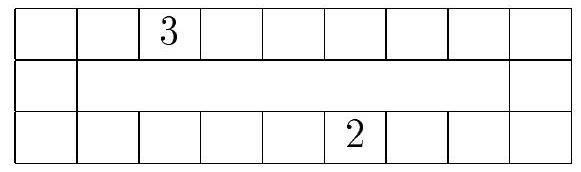
\includegraphics[max width=\textwidth, center]{2024_11_21_1a8d26d2d1f00028bc7ag-1}


\end{document}